\documentclass{standalone}
\usepackage{tikz}
\usetikzlibrary{patterns, positioning}
\usepackage[sfdefault]{ClearSans} %% option 'sfdefault' activates Clear Sans as the default text font
\usepackage[T1]{fontenc}

\begin{document}
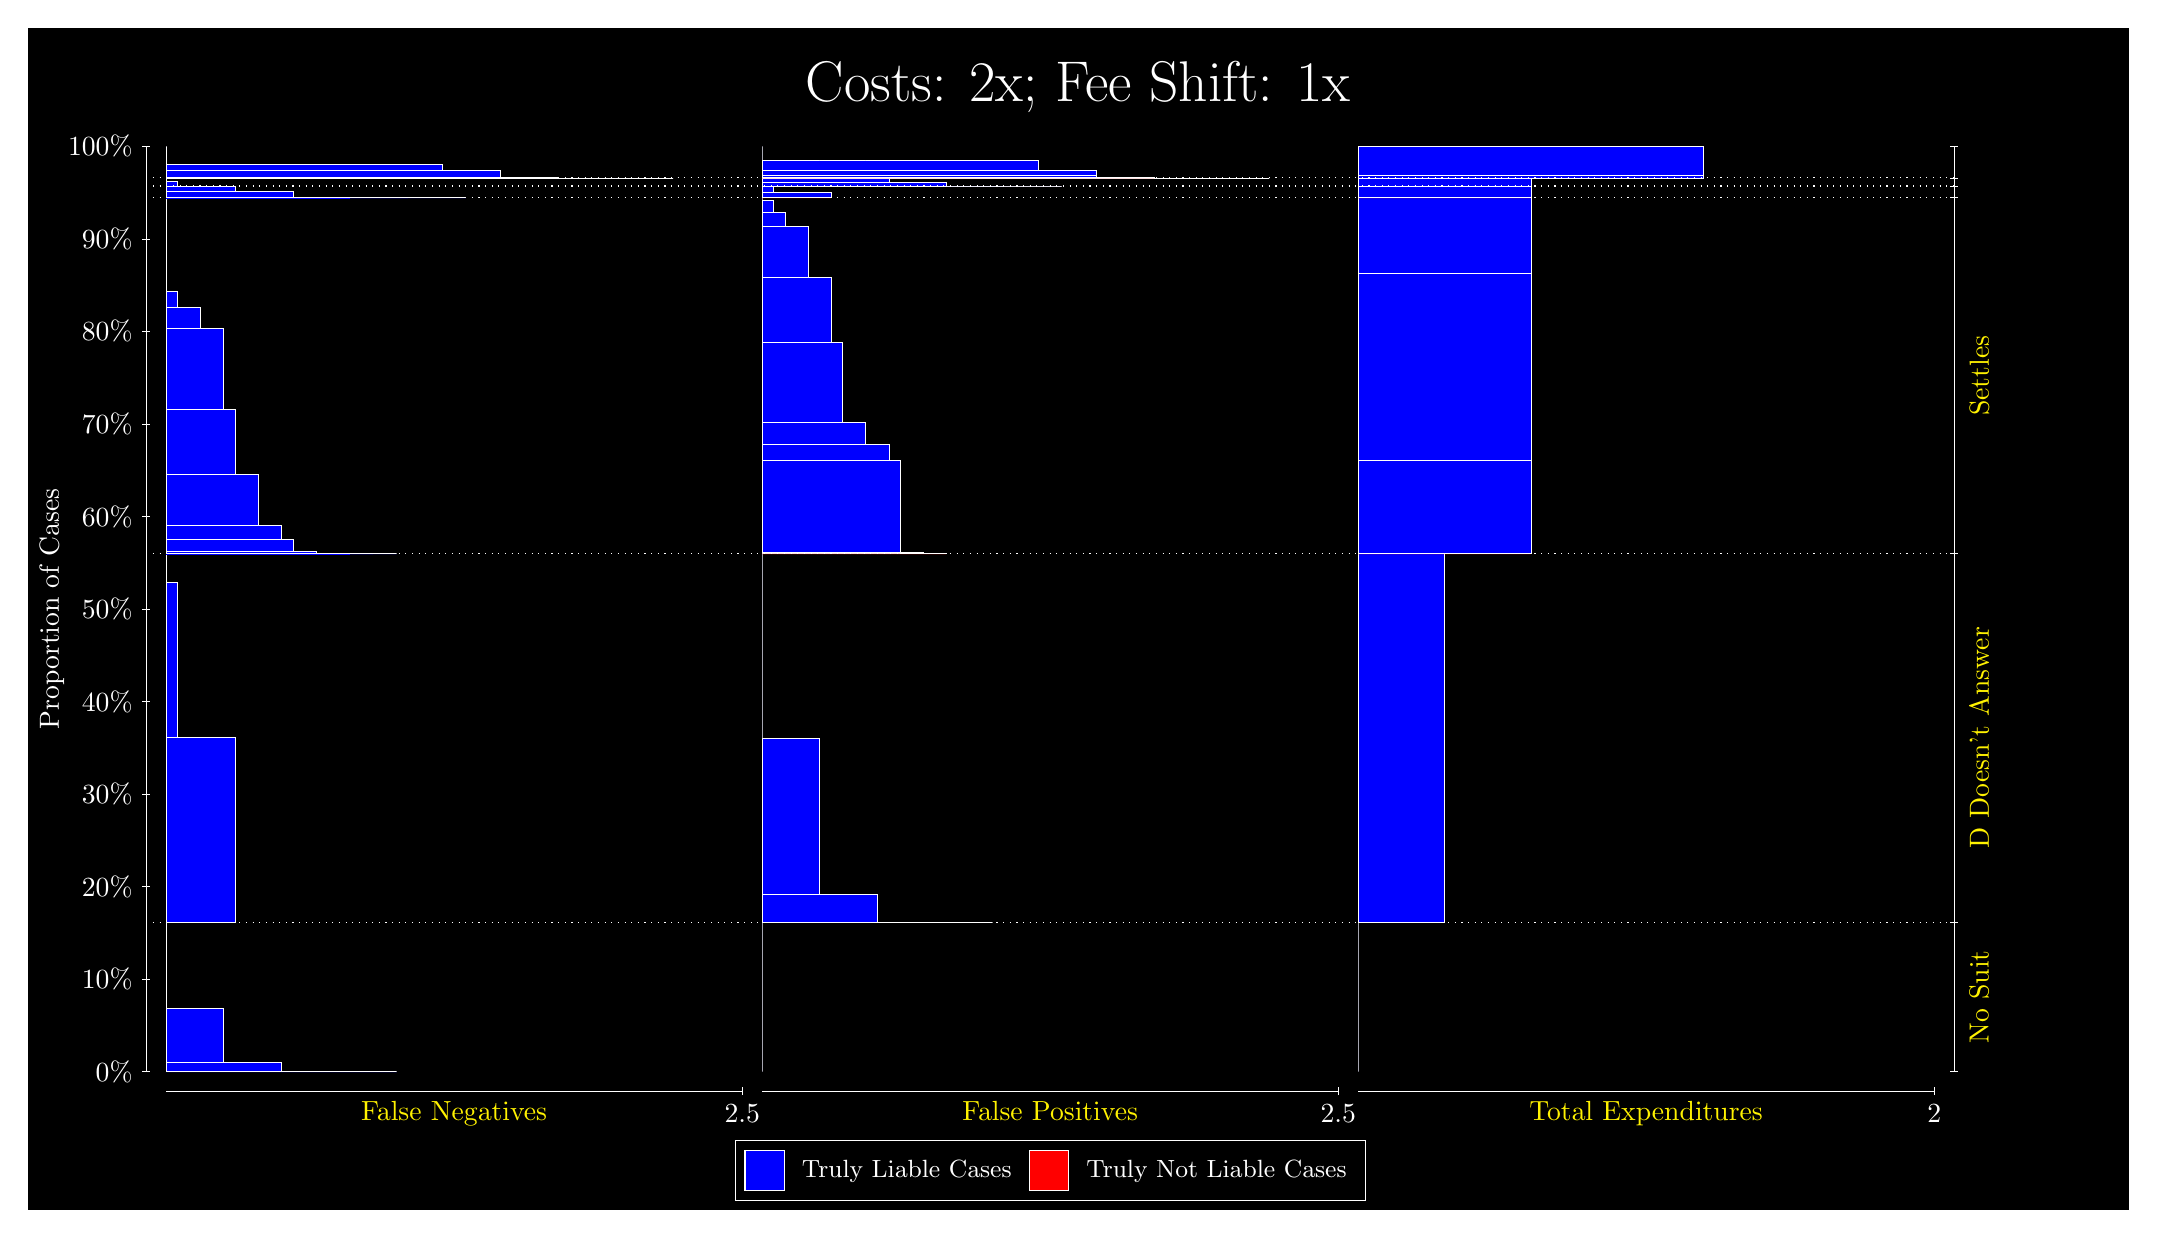
\begin{tikzpicture}
\draw[fill=black] (0,0) rectangle (26.667,15);
\draw[text=white] (0,13.5) rectangle (26.667,15) node[midway] {\huge Costs: 2x; Fee Shift: 1x};
\draw[white, very thin] (1.5,1.75) -- (1.5,13.5);
\node[rotate=90, text=white, anchor=center] at (0.3, 7.625) {Proportion of Cases};
\draw[white, very thin] (1.45,1.75) -- (1.55,1.75);
\node[text=white, anchor=east] at (1.45, 1.75) {0\%};
\draw[white, very thin] (1.45,2.925) -- (1.55,2.925);
\node[text=white, anchor=east] at (1.45, 2.925) {10\%};
\draw[white, very thin] (1.45,4.1) -- (1.55,4.1);
\node[text=white, anchor=east] at (1.45, 4.1) {20\%};
\draw[white, very thin] (1.45,5.275) -- (1.55,5.275);
\node[text=white, anchor=east] at (1.45, 5.275) {30\%};
\draw[white, very thin] (1.45,6.45) -- (1.55,6.45);
\node[text=white, anchor=east] at (1.45, 6.45) {40\%};
\draw[white, very thin] (1.45,7.625) -- (1.55,7.625);
\node[text=white, anchor=east] at (1.45, 7.625) {50\%};
\draw[white, very thin] (1.45,8.8) -- (1.55,8.8);
\node[text=white, anchor=east] at (1.45, 8.8) {60\%};
\draw[white, very thin] (1.45,9.975) -- (1.55,9.975);
\node[text=white, anchor=east] at (1.45, 9.975) {70\%};
\draw[white, very thin] (1.45,11.15) -- (1.55,11.15);
\node[text=white, anchor=east] at (1.45, 11.15) {80\%};
\draw[white, very thin] (1.45,12.325) -- (1.55,12.325);
\node[text=white, anchor=east] at (1.45, 12.325) {90\%};
\draw[white, very thin] (1.45,13.5) -- (1.55,13.5);
\node[text=white, anchor=east] at (1.45, 13.5) {100\%};

\draw[white, very thin] (24.457,1.75) -- (24.457,13.5);
\draw[white, very thin] (24.407,1.75) -- (24.507,1.75);
\node[anchor=west] at (24.407, 1.75) {};
\draw[white, very thin] (24.407,3.6473) -- (24.507,3.6473);
\node[anchor=west] at (24.407, 3.6473) {};
\draw[white, very thin] (24.407,8.3258) -- (24.507,8.3258);
\node[anchor=west] at (24.407, 8.3258) {};
\draw[white, very thin] (24.407,12.849) -- (24.507,12.849);
\node[anchor=west] at (24.407, 12.849) {};
\draw[white, very thin] (24.407,12.996) -- (24.507,12.996);
\node[anchor=west] at (24.407, 12.996) {};
\draw[white, very thin] (24.407,13.1) -- (24.507,13.1);
\node[anchor=west] at (24.407, 13.1) {};
\draw[white, very thin] (24.407,13.5) -- (24.507,13.5);
\node[anchor=west] at (24.407, 13.5) {};

\draw[white, very thin, fill=blue] (1.75,1.75) rectangle (4.6775,1.75);
\draw[white, very thin, fill=blue] (1.75,1.75) rectangle (3.9457,1.751);
\draw[white, very thin, fill=blue] (1.75,1.751) rectangle (3.2138,1.8683);
\draw[white, very thin, fill=blue] (1.75,1.8683) rectangle (2.4819,2.5563);
\draw[white, very thin, fill=red] (1.75,2.5563) rectangle (1.75,2.5563);
\draw[white, very thin, fill=blue] (1.75,2.5563) rectangle (1.75,3.6473);
\draw[white, very thin, fill=blue] (1.75,3.6473) rectangle (2.6283,5.9935);
\draw[white, very thin, fill=blue] (1.75,5.9935) rectangle (1.8964,7.9693);
\draw[white, very thin, fill=red] (1.75,7.9693) rectangle (1.75,7.9693);
\draw[white, very thin, fill=blue] (1.75,7.9693) rectangle (1.75,8.3258);
\draw[white, very thin, fill=blue] (1.75,8.3258) rectangle (4.6775,8.3258);
\draw[white, very thin, fill=blue] (1.75,8.3258) rectangle (4.3848,8.3258);
\draw[white, very thin, fill=blue] (1.75,8.3258) rectangle (4.092,8.3262);
\draw[white, very thin, fill=blue] (1.75,8.3262) rectangle (3.9457,8.3274);
\draw[white, very thin, fill=blue] (1.75,8.3274) rectangle (3.6529,8.354);
\draw[white, very thin, fill=blue] (1.75,8.354) rectangle (3.3602,8.5142);
\draw[white, very thin, fill=blue] (1.75,8.5142) rectangle (3.2138,8.6894);
\draw[white, very thin, fill=blue] (1.75,8.6894) rectangle (2.921,9.3343);
\draw[white, very thin, fill=blue] (1.75,9.3343) rectangle (2.6283,10.162);
\draw[white, very thin, fill=blue] (1.75,10.162) rectangle (2.4819,11.185);
\draw[white, very thin, fill=blue] (1.75,11.185) rectangle (2.1891,11.462);
\draw[white, very thin, fill=blue] (1.75,11.462) rectangle (1.8964,11.659);
\draw[white, very thin, fill=red] (1.75,11.659) rectangle (1.75,11.659);
\draw[white, very thin, fill=blue] (1.75,11.659) rectangle (1.75,12.849);
\draw[white, very thin, fill=blue] (1.75,12.849) rectangle (5.5558,12.849);
\draw[white, very thin, fill=blue] (1.75,12.849) rectangle (4.8239,12.849);
\draw[white, very thin, fill=blue] (1.75,12.849) rectangle (4.092,12.85);
\draw[white, very thin, fill=blue] (1.75,12.85) rectangle (3.3602,12.928);
\draw[white, very thin, fill=blue] (1.75,12.928) rectangle (2.6283,12.996);
\draw[white, very thin, fill=red] (1.75,12.996) rectangle (1.75,12.996);
\draw[white, very thin, fill=blue] (1.75,12.996) rectangle (2.6283,12.997);
\draw[white, very thin, fill=blue] (1.75,12.997) rectangle (1.8964,13.057);
\draw[white, very thin, fill=red] (1.75,13.057) rectangle (1.75,13.057);
\draw[white, very thin, fill=blue] (1.75,13.057) rectangle (1.75,13.1);
\draw[white, very thin, fill=blue] (1.75,13.1) rectangle (8.1906,13.1);
\draw[white, very thin, fill=blue] (1.75,13.1) rectangle (7.4587,13.1);
\draw[white, very thin, fill=blue] (1.75,13.1) rectangle (6.7268,13.107);
\draw[white, very thin, fill=blue] (1.75,13.107) rectangle (5.9949,13.199);
\draw[white, very thin, fill=blue] (1.75,13.199) rectangle (5.2631,13.275);
\draw[white, very thin, fill=blue] (1.75,13.275) rectangle (4.5312,13.275);
\draw[white, very thin, fill=blue] (1.75,13.275) rectangle (3.9457,13.275);
\draw[white, very thin, fill=blue] (1.75,13.275) rectangle (3.7993,13.275);
\draw[white, very thin, fill=blue] (1.75,13.275) rectangle (3.2138,13.275);
\draw[white, very thin, fill=blue] (1.75,13.275) rectangle (2.4819,13.276);
\draw[white, very thin, fill=red] (1.75,13.276) rectangle (1.75,13.276);
\draw[white, very thin, fill=blue] (1.75,13.276) rectangle (1.75,13.5);
\draw[white, very thin, fill=red] (9.3189,1.75) rectangle (9.3189,1.75);
\draw[white, very thin, fill=blue] (9.3189,1.75) rectangle (9.3189,3.6473);
\draw[white, very thin, fill=red] (9.3189,3.6473) rectangle (12.246,3.6473);
\draw[white, very thin, fill=blue] (9.3189,3.6473) rectangle (12.246,3.6473);
\draw[white, very thin, fill=blue] (9.3189,3.6473) rectangle (11.515,3.6496);
\draw[white, very thin, fill=blue] (9.3189,3.6496) rectangle (10.783,4.0038);
\draw[white, very thin, fill=blue] (9.3189,4.0038) rectangle (10.051,5.9796);
\draw[white, very thin, fill=blue] (9.3189,5.9796) rectangle (9.3189,8.3258);
\draw[white, very thin, fill=red] (9.3189,8.3258) rectangle (11.661,8.3258);
\draw[white, very thin, fill=blue] (9.3189,8.3258) rectangle (11.661,8.3307);
\draw[white, very thin, fill=red] (9.3189,8.3307) rectangle (11.368,8.3307);
\draw[white, very thin, fill=blue] (9.3189,8.3307) rectangle (11.368,8.3381);
\draw[white, very thin, fill=red] (9.3189,8.3381) rectangle (11.075,8.3381);
\draw[white, very thin, fill=blue] (9.3189,8.3381) rectangle (11.075,9.5153);
\draw[white, very thin, fill=blue] (9.3189,9.5153) rectangle (10.929,9.7127);
\draw[white, very thin, fill=blue] (9.3189,9.7127) rectangle (10.636,9.9892);
\draw[white, very thin, fill=blue] (9.3189,9.9892) rectangle (10.344,11.012);
\draw[white, very thin, fill=blue] (9.3189,11.012) rectangle (10.197,11.84);
\draw[white, very thin, fill=blue] (9.3189,11.84) rectangle (9.9044,12.485);
\draw[white, very thin, fill=blue] (9.3189,12.485) rectangle (9.6116,12.66);
\draw[white, very thin, fill=blue] (9.3189,12.66) rectangle (9.4652,12.82);
\draw[white, very thin, fill=blue] (9.3189,12.82) rectangle (9.3189,12.849);
\draw[white, very thin, fill=red] (9.3189,12.849) rectangle (10.197,12.849);
\draw[white, very thin, fill=blue] (9.3189,12.849) rectangle (10.197,12.916);
\draw[white, very thin, fill=blue] (9.3189,12.916) rectangle (9.4652,12.994);
\draw[white, very thin, fill=blue] (9.3189,12.994) rectangle (9.3189,12.996);
\draw[white, very thin, fill=red] (9.3189,12.996) rectangle (13.125,12.996);
\draw[white, very thin, fill=blue] (9.3189,12.996) rectangle (13.125,12.996);
\draw[white, very thin, fill=blue] (9.3189,12.996) rectangle (12.393,12.996);
\draw[white, very thin, fill=blue] (9.3189,12.996) rectangle (11.661,13.039);
\draw[white, very thin, fill=blue] (9.3189,13.039) rectangle (10.929,13.099);
\draw[white, very thin, fill=blue] (9.3189,13.099) rectangle (10.197,13.1);
\draw[white, very thin, fill=red] (9.3189,13.1) rectangle (15.759,13.1);
\draw[white, very thin, fill=blue] (9.3189,13.1) rectangle (15.759,13.1);
\draw[white, very thin, fill=blue] (9.3189,13.1) rectangle (15.028,13.1);
\draw[white, very thin, fill=red] (9.3189,13.1) rectangle (15.028,13.1);
\draw[white, very thin, fill=blue] (9.3189,13.1) rectangle (15.028,13.1);
\draw[white, very thin, fill=blue] (9.3189,13.1) rectangle (14.296,13.104);
\draw[white, very thin, fill=red] (9.3189,13.104) rectangle (14.296,13.104);
\draw[white, very thin, fill=blue] (9.3189,13.104) rectangle (14.296,13.106);
\draw[white, very thin, fill=blue] (9.3189,13.106) rectangle (13.564,13.136);
\draw[white, very thin, fill=red] (9.3189,13.136) rectangle (13.564,13.136);
\draw[white, very thin, fill=blue] (9.3189,13.136) rectangle (13.564,13.199);
\draw[white, very thin, fill=blue] (9.3189,13.199) rectangle (12.832,13.2);
\draw[white, very thin, fill=blue] (9.3189,13.2) rectangle (12.832,13.324);
\draw[white, very thin, fill=blue] (9.3189,13.324) rectangle (12.1,13.325);
\draw[white, very thin, fill=blue] (9.3189,13.325) rectangle (11.368,13.325);
\draw[white, very thin, fill=red] (9.3189,13.325) rectangle (10.783,13.325);
\draw[white, very thin, fill=blue] (9.3189,13.325) rectangle (10.783,13.325);
\draw[white, very thin, fill=blue] (9.3189,13.325) rectangle (10.636,13.325);
\draw[white, very thin, fill=red] (9.3189,13.325) rectangle (10.051,13.325);
\draw[white, very thin, fill=blue] (9.3189,13.325) rectangle (10.051,13.325);
\draw[white, very thin, fill=red] (9.3189,13.325) rectangle (9.3189,13.325);
\draw[white, very thin, fill=blue] (9.3189,13.325) rectangle (9.3189,13.5);
\draw[white, very thin, fill=red] (16.888,1.75) rectangle (16.888,1.75);
\draw[white, very thin, fill=blue] (16.888,1.75) rectangle (16.888,3.6473);
\draw[white, very thin, fill=red] (16.888,3.6473) rectangle (17.986,3.6473);
\draw[white, very thin, fill=blue] (16.888,3.6473) rectangle (17.986,8.3258);
\draw[white, very thin, fill=red] (16.888,8.3258) rectangle (19.083,8.3258);
\draw[white, very thin, fill=blue] (16.888,8.3258) rectangle (19.083,9.5164);
\draw[white, very thin, fill=red] (16.888,9.5164) rectangle (19.083,9.5164);
\draw[white, very thin, fill=blue] (16.888,9.5164) rectangle (19.083,11.893);
\draw[white, very thin, fill=red] (16.888,11.893) rectangle (19.083,11.893);
\draw[white, very thin, fill=blue] (16.888,11.893) rectangle (19.083,12.849);
\draw[white, very thin, fill=red] (16.888,12.849) rectangle (19.083,12.849);
\draw[white, very thin, fill=blue] (16.888,12.849) rectangle (19.083,12.996);
\draw[white, very thin, fill=red] (16.888,12.996) rectangle (19.083,12.996);
\draw[white, very thin, fill=blue] (16.888,12.996) rectangle (19.083,13.1);
\draw[white, very thin, fill=red] (16.888,13.1) rectangle (21.279,13.1);
\draw[white, very thin, fill=blue] (16.888,13.1) rectangle (21.279,13.135);
\draw[white, very thin, fill=red] (16.888,13.135) rectangle (21.279,13.135);
\draw[white, very thin, fill=blue] (16.888,13.135) rectangle (21.279,13.5);
\draw[white, dotted] (1.5,3.6473) -- (24.457,3.6473);
\draw[white, dotted] (1.5,8.3258) -- (24.457,8.3258);
\draw[white, dotted] (1.5,12.849) -- (24.457,12.849);
\draw[white, dotted] (1.5,12.996) -- (24.457,12.996);
\draw[white, dotted] (1.5,13.1) -- (24.457,13.1);
\draw[white, very thin] (1.75,1.5) -- (9.0689,1.5);
\node[text=yellow, anchor=north] at (5.4094, 1.5) {False Negatives};
\draw[white, very thin] (9.0689,1.45) -- (9.0689,1.55);
\node[text=white, anchor=north] at (9.0689, 1.45) {2.5};

\draw[white, very thin] (9.3189,1.5) -- (16.638,1.5);
\node[text=yellow, anchor=north] at (12.978, 1.5) {False Positives};
\draw[white, very thin] (16.638,1.45) -- (16.638,1.55);
\node[text=white, anchor=north] at (16.638, 1.45) {2.5};

\draw[white, very thin] (16.888,1.5) -- (24.207,1.5);
\node[text=yellow, anchor=north] at (20.547, 1.5) {Total Expenditures};
\draw[white, very thin] (24.207,1.45) -- (24.207,1.55);
\node[text=white, anchor=north] at (24.207, 1.45) {2};

\node[text=yellow, centered, rotate=90] at (24.777, 2.6987) {No Suit};
\node[text=yellow, centered, rotate=90] at (24.777, 5.9865) {D Doesn't Answer};
\node[text=yellow, centered, rotate=90] at (24.777, 10.587) {Settles};




\draw (12.978300999999998,1.5) node[draw=none] (baseCoordinate) {};
\begin{scope}[align=center]
        \matrix[scale=0.5, draw=white, below=0.5cm of baseCoordinate, nodes={draw}, column sep=0.1cm]{
            \node[rectangle, draw, minimum width=0.5cm, minimum height=0.5cm, fill=blue] {}; &
            \node[draw=none, font=\small, text=white] (B) {Truly Liable Cases}; &
            \node[rectangle, draw, minimum width=0.5cm, minimum height=0.5cm, fill=red] {}; &
            \node[draw=none, font=\small, text=white] (B) {Truly Not Liable Cases}; \\
            };
\end{scope}

\end{tikzpicture}
\end{document}